\documentclass{sig-alternate}
\usepackage[english]{babel}
\usepackage{float}
\usepackage{graphicx}
\usepackage{xcolor}
\usepackage{minted}
\usemintedstyle[html]{borland}
\usemintedstyle[common-lisp]{pastie}
\bibliographystyle{abbrv}

\begin{document}

\setcopyright{rightsretained}
\doi{}
\isbn{}
\conferenceinfo{ELS'17}{April 3--4, 2017, Brussel, Belgium}

\begin{CCSXML}
<ccs2012>
  <concept>
    <concept_id>10011007.10011006.10011066</concept_id>
    <concept_desc>Software and its engineering~Development frameworks and environments</concept_desc>
    <concept_significance>500</concept_significance>
  </concept>
  <concept>
    <concept_id>10002951.10003260.10003282</concept_id>
    <concept_desc>Information systems~Web applications</concept_desc>
    <concept_significance>300</concept_significance>
  </concept>
</ccs2012>
\end{CCSXML}

\ccsdesc[500]{Software and its engineering~Development frameworks and environments}
\ccsdesc[300]{Information systems~Web applications}

\title{Radiance - A Web Application Environment}

\numberofauthors{1}
\author{
\alignauthor
Nicolas Hafner\\
       \affaddr{Shirakumo.org}\\
       \affaddr{Zürich, Switzerland}\\
       \email{shinmera@tymoon.eu}
}
\date{15 November 2016}

\maketitle

\begin{abstract}
  Radiance\cite{radiance} is a set of libraries that provides an environment for web applications. Unlike traditional web frameworks that focus on a set of tools to support the construction and maintenance of a single application, Radiance attempts to allow one to run as many differing applications as desired in the same environment. This goal brings many advantages, as frequently there are common resources in applications that should be shared between them, but cannot, because the applications are separated and developed without regard for sharing. In order to fix this, Radiance provides an extensible interface mechanism to standardise the interaction between users of common resources. To facilitate the separation and encapsulation of the shared URL address space between applications, Radiance also provides a flexible routing mechanism. This mechanism is powerful enough to ensure that any application written with Radiance can be deployed on a server setup, no matter how complicated the constraints, without needing to change the source code of the application.
\end{abstract}

\printccsdesc

\keywords{Common Lisp, web framework, web development, encapsulation, interfacing}
\newpage

\section{Introduction}
Most tasks involved in writing a website or web application are not very complex or complicated; they usually involve solving very similar problems every time. This trend lead to the rise of web frameworks-- collections of tools and libraries to take care of the most common of aspects for the developer. \\

A web application framework is comprised of several components. This can go from the absolute minimum of an HTTP server and URL dispatch mechanism as seen in microframeworks\cite{microframeworks}, to a vast range of tools including database access, authentication, user management, validation, API endpoints, and more. All of these components exist with the aim of reducing the amount of work necessary to write a single web application. \\

Usually these frameworks have the goal of supporting developers in writing a single, particular application. This can lead to issues when the application is supposed to be deployed on wildly different setups than it was developed on, or if it should share the space with other applications. Solutions to resource sharing or configuration then have to be designed by the application itself, and are thus often ad-hoc and incompatible with other applications. As an example, even if you have two applications like a forum and a blog that were both written with the same framework, they are usually deployed in such a format, that you won't feasibly be able to configure your system to allow both to share the same login and account information, or other kinds of data. \\

This leads to a frustrating experience for the administrator of a server setup, who either has to go through complicated deployment and configuration steps to bend the applications to fit his requirements, or even has to go so far as to change the source code to do what he needs.

\section{Radiance's Approach}
Radiance was designed with a different perspective in mind. Instead of viewing the application design process through the lens of the developer, it looks at it from the view of an administrator that would like to run an application on one of his servers. Doing so allowed it to come up with solutions to these problems that can simultaneously account for the needs of an administrator, and those of a developer. For example, an administrator may want to configure which database and server to use, confine an application to a particular domain or path, or share a domain across multiple applications. \\

\subsection{Interfaces}
The first piece that came out of this line of thinking is an interface system. This system allows the specification of signatures of a package. What this means is that functions, macros, variables, etc. are defined in their signature only, without any actual functionality being implemented that makes them work. For example, a simplified interface to a database might look like this:

\begin{minted}[fontsize=\small]{common-lisp}
(define-interface database
  (defun select (table where &key limit skip sort))
  (defun insert (table data))
  (defun delete (table where &key limit skip sort))
  (defun update (table data where &key limit skip sort))
  (defmacro with-transaction ((name) &body body)))
\end{minted}

While the example here only shows the definition of functions and a macro, it is possible to extend the system to any definition facility desired. The description of the general behaviour of each of these definitions cannot be expressed in code however, and must be specified in documentation. \\

Applications can now make use of this interface and write code against it. As long as the use corresponds to the specified signatures and behaviour, the code is promised to work correctly. \\

The code that actually realises the specific behaviour of the individual definitions is left up to an implementation of the respective interface. Such an implementation can be a regular system that simply overwrites the stubs defined by the interface. In the case of our proposed database interface, we could have multiple implementations to choose from, each of which provides the glue code to a particular type of database system. The choice of the specific implementation for an interface is left up to the administrator of a Radiance installation. Since the applications that make use of an interface and the implementation for it must conform to its specified behaviour, all applications should work regardless of the particular implementation chosen. \\

Radiance provides standard interface definitions for most of the common aspects of web application programming, allowing the sharing of the previously discussed common resources. However, it is also sensible to define interfaces for commonly needed tools that may have slightly different implementation details. An example for this would be a caching system; the exact behaviour of the cache can vary --be it database-backed, file-backed, memory-backed, etc.-- but the usage of the system is the same, regardless of implementation details. \\

Specifically, Radiance defines standard interfaces for banning, rate-limiting, an administration panel, caching, authentication, sessions, users, user profiles, the HTTP server, logging, database interaction, and database record abstraction. While the interface definitions will always be around, not every interface needs to load an implementation unless there is an application that specifically requests it. Thus, the amount of functionality Radiance provides is also dynamic and without penalty for minimal setups. \\

Since the implementation mechanism does not rely on some sort of indirection facility, interface functionality incurs zero overhead, allowing implementations to be as efficient as possible. This advantage is one of the details of the system that are rather specific to Lisp, since it makes this kind of behaviour trivial to implement. \\

Thus, the interface mechanism solves the problem of shared access across applications without constraining the system to a particular implementation. Thanks to this, the administrator of the system can choose the appropriate implementation for his setup, without having to take care to respect the wishes of every application. \\

\subsection{Routing}
The second piece is a powerful routing system. While most frameworks seem to conflate routing and dispatching, Radiance makes a clear distinction. Dispatching is the process of determining which function should provide the response to a request to a particular URL. Routing is the process of transforming a URL in some fashion, thus ``routing'' it somewhere else. \\

The routing system lies between the HTTP server and the web applications, leading to the following request lifecycle for a typical Radiance setup: \\

\begin{figure}[H]
  \centering
  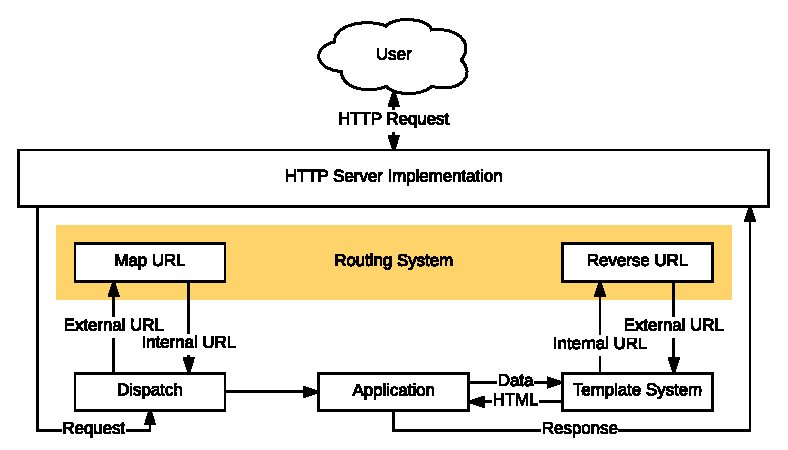
\includegraphics[width=0.5\textwidth]{request.pdf}
  \caption{Radiance Request Lifecycle}
\end{figure}

The URL on which the request arrives is transformed into an internal representation by so-called ``mapping routes''. This internal representation, called a ``URI'', is composed of a list of subdomains, an optional port, and a path string. The other information contained in a URL is not necessary for routing or dispatching. Then the request is dispatched to the first handler that matches the URI. It can decide what to do with it, which is usually to render some kind of template. In order to ensure that links and references within the emitted HTML can actually be resolved, the template system must use URIs that are translated by so-called ``reversal routes'' to produce a URL. The completed HTML document is then sent back as a response to the request. \\

The routing system is thus responsible for maintaining the separation of the system into two different worlds: an external one that the server and users of the site interact with, and an internal one that applications deal with. \\

As an example, let us imagine a server set up on \\ \texttt{radiance.example.com/test/} that runs a single application. The application will be called ``hello'' and has the following code to define a page:

\begin{minted}{common-lisp}
(define-page index "hello/index" ()
  (r-clip:process (@template "index.ctml")))
\end{minted}

If an (untranslated) request to \texttt{hello/index} were performed, the above code will be executed, and the template system Clip\cite{clip} will render the \texttt{index.ctml} file. The template might look as follows:

\begin{minted}{html}
<link rel="stylesheet" type="text/css"
      @href="hello/static/hello/index.css" />
<h1>Hello!</h1>
\end{minted}

Clip will recognise the \texttt{@href} attribute, parse its value as a URI, send it through the reversal routes, and set the resulting URL as the value for the \texttt{href} attribute. Thus, the cycle illustrated in Figure 1 is followed by our minimal setup here. \\

As it stands, Radiance would translate a request to \\\texttt{http://radiance.example.com/test/index} into the URI \\\texttt{radiance.example.com/test/index} and then map it to \\\texttt{radiance/test/index}. The top-level domain --the part of the domain we cannot change-- is stripped away by one of the standard routes. This URI is still not one that would invoke our page though. Therefore, additional routes need to be set up to handle the conversion to and from the internal representation.

\begin{minted}{common-lisp}
(define-string-route index :mapping 
  "radiance/test/(.*)" "hello/\\1")
(define-string-route index :reversal
  "hello/(.*)" "radiance/test/\\1")
\end{minted}

With these routes in place, our previous example URL will be mapped to \texttt{hello/index} as required. Furthermore, the requested reversal of the URI \texttt{/static/hello/index.css} within the template will be turned into the URL \\\texttt{\small http://radiance.example.com/test/static/hello/index.css},\\ completing the cycle properly. The top-level domain here is reattached by another standard route. \\

While the above routes are fairly simplistic in their behaviour, routes can be written to perform arbitrary operations, including stashing away data for later use during reversal. This flexibility allows things like the virtual subdomain route that is included by default. This route recognises when a request like this \texttt{/!/subdomain/foo} and maps it to \texttt{subdomain/foo}. It is necessary for the corresponding reversal route to know that the initial request was mapped by this particular route in order to appropriately translate back to the prefix, as there is no indication in the URI that we want to reverse that this should happen. The virtual domain routing is especially useful on development setups, where no real domains are directly available. It allows you to use \texttt{localhost} or even just the IP address to reach everything. \\

In order for everything to fit together, applications need to abide by some conventions that Radiance postulates. The most important one is that each application gets its own subdomain in the internal representation. This convention allows applications to assume that they have free reign over the path part of the URL. Additionally, the path prefixes \texttt{/static/} and \texttt{/api/} are reserved by Radiance on all domains, and are used to provide static files and REST api endpoints respectively. This way, routes can be written in a more generic manner to solve common problems, rather than requiring specifically tailored rules for each application. \\

Thus, providing a generic translation mechanism for URLs allows applications to be written in a way that prevents them from clashing with each other, while at the same time gaining the ability for administrators to configure the URL namespace according to their constraints and needs. \\

\subsection{Resources}
The final piece is a generic resource mechanism that allows the exchange of information between applications, and particularly between applications and interface implementations. This piece is necessary because applications may need to refer to resources provided by other components in the Radiance environment. For example, the login page and mechanism is provided by the authentication interface. An application may want to present a link to this page to the users. However, because the location of this page is not standardised, the application has no direct way of knowing where the page would be. Instead of specifying the page location, Radiance provides a system that allows the retrieval of such resources generically. \\

Several standard resource types are specified, though more can be defined by an application writer; for example to provide for an extension mechanism. The most important standard resource type is the \texttt{page}, which returns a URI to a requested page, if it exists. Thus, a code like the following will produce a URL to the login screen of the authentication interface:

\begin{minted}{common-lisp}
(uri-to-url (resource :auth :page "login")
            :representation :external)
\end{minted}

The interface definitions are extended to allow expressing that an implementation must provide for a particular resource, providing the above behaviour as a promise.

\section{Conclusions}
By implementing the components presented in this paper, Radiance allows for an environment that can conveniently house multiple applications in the same Lisp process. It seamlessly handles both the sharing of common resources, as well as the encapsulation and separation of each application. In order to make it feasible for every application to run on any target setup, and to make it adaptable to an administrator's requirements for the public web interface, a powerful routing system was created that not only handles the incoming request, but also the outgoing data. \\

These components present clear advantages to the administrator of a system and to the developer of an application, as they simplify and streamline various parts that would otherwise be implemented ad-hoc. Particularly, development and production setups can both be configured with ease.

\bibliography{paper}
\end{document}

%%% Local Variables:
%%% mode: latex
%%% TeX-command-extra-options: "-shell-escape"
%%% TeX-master: t
%%% TeX-engine: luatex
%%% End:
